\section{Microcontroller Design}

We present four implementations of \textsf{FrodoKEM}. We implemented both parameter sets \textsf{FrodoKEM-640} and \textsf{FrodoKEM-976}
and we also implemented both possible pseudo-random numbers generators for the generation of $\mathbf{A}$. For AES, we rely on the optimized implementation by Schwabe and Stoffelen \cite{DBLP:conf/sacrypt/SchwabeS16} and for cSHAKE we use the assembly implementation from the official KECCAK code package \cite{bertoni2016keccak}.

\subsection{Target Platform}

We evaluate our microcontroller implementation of \textsf{FrodoKEM} on the STM32F407 Discovery board that has a 32-bit ARM Cortex-M4F microprocessor that runs with up to 168 MHz. Our development board comes with 192 kilobyte of RAM and one megabyte of Flash memory. Furthermore the Cortex-M4 features powerful DSP instructions like single-cycle multiply-with-accumulate and a true random number generator based on analog noise. However, in contrast to other M4-based microcontrollers, our development board does not have an AES-accelerator that could be used to speed-up \textsf{FrodoKEM-AES}. As development environment we use CooCox CoIDE version 1.7.7 with gcc-arm-none-eabi 5.4 2016 toolchain. The Cortex-M4F has 13 general purpose registers and ($R0-R12$), one register reserved for the stack pointer, a link register, one register reserved for the program counter, and special-purpose program status registers. When mixing C with assembly it is important to note that the calling convention requires parameters to be in $R0-R3$ and the result to be in $R0-R1$. The link register can be used as general purpose register as well, if the assembly function does not call any other function and its original value is restored before leaving the function.

\subsection{High-level Memory Optimization}

The official specification of \textsf{FrodoKEM} reports a peak stack memory usage of 189,176 bytes for \textsf{FrodoKEM-976-AES}. As our microcontroller has only access to 192 kilobytes of RAM, we carefully analyze the memory allocation of the reference implementation to see whether we can make the implementation more efficient in terms of memory usage. Keep in mind that for many applications there is another software running beside the KEM, therefore it is sensible to reduce the memory consumption as much as possible without sacrificing performance. With the help of the flow chart of the most important operations in \textsf{FrodoKEM} (Figure \ref{fig:flowchart_encaps} and \ref{fig:flowchart_decaps}), it is easily possible to see which matrices are used for which computations. The highlighted intermediate values are large arrays with $n \times \bar{n}$ elements. As we store each element in two bytes, this means that one large array requires $976 \times 8 \times 2 = 15,616$ bytes of RAM for each large array for \textsf{FrodoKEM-976-AES}. The non-highlighted intermediate values are small ($\bar{n} \times \bar{n}$ elements, i.e. 128 bytes) and therefore we focus on optimizing the large ones. 

The first thing to note about decapsulation, as shown in Figure \ref{fig:flowchart_decaps}, is that we need memory for at least two large arrays. For instance, during the computation of $\mathbf{B}''$, both inputs $\mathbf{E'}$ and $\mathbf{S'}$ are large. While $\mathbf{E'}$ can be generated on the fly, $\mathbf{S'}$ is loaded multiple times during the multiplication by $\mathbf{A}$ and therefore on-the-fly computation would imply regenerating the same value over and over again. Therefore we decided that the better trade-off would be to keep storage space for at least two large arrays. Another thing to note is that the right-hand side can be computed completely independent from the left-hand side. Therefore we can store $\mathbf{S'}$ in one of our two memory slots for large arrays and compute $\mathbf{V}$ and $\mathbf{B''}$ using the other memory slot. Once $\mathbf{V}$ and $\mathbf{B''}$ are calculated, $\mathbf{S'}$ is no longer used and can be replaced by $\mathbf{B'}$.

In the flow chart of encapsulation in Figure \ref{fig:flowchart_encaps} we can see that two large arrays are also sufficient for the encapsulation as the sampling of $\mathbf{E'}$ and the unpacking of $\mathbf{B}$ can be done on-the-fly. In fact the encapsulation needs even less memory as for instance the packing of $\mathbf{B'}$ could be done on-the-fly as well. But as the bottleneck in terms of memory consumption is the decapsulation, we do not further optimize the encapsulation.

\begin{figure*}[tbhp]
\centering

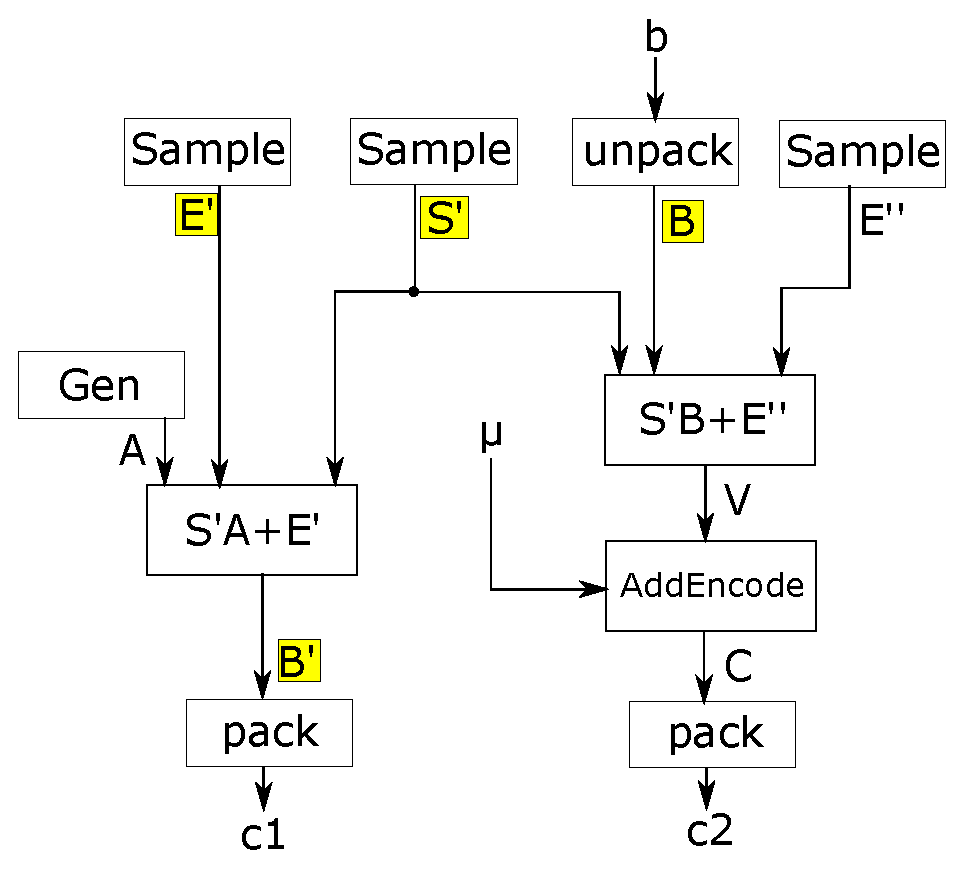
\includegraphics[scale=0.6]{figures/frodo_flowchart_encaps}

\caption{Flowchart of the encapsulation. Yellow highlighted matrices are $n \times \bar{n}$ matrices.}
\label{fig:flowchart_encaps}
\end{figure*}

\begin{figure*}[tbhp]
\centering

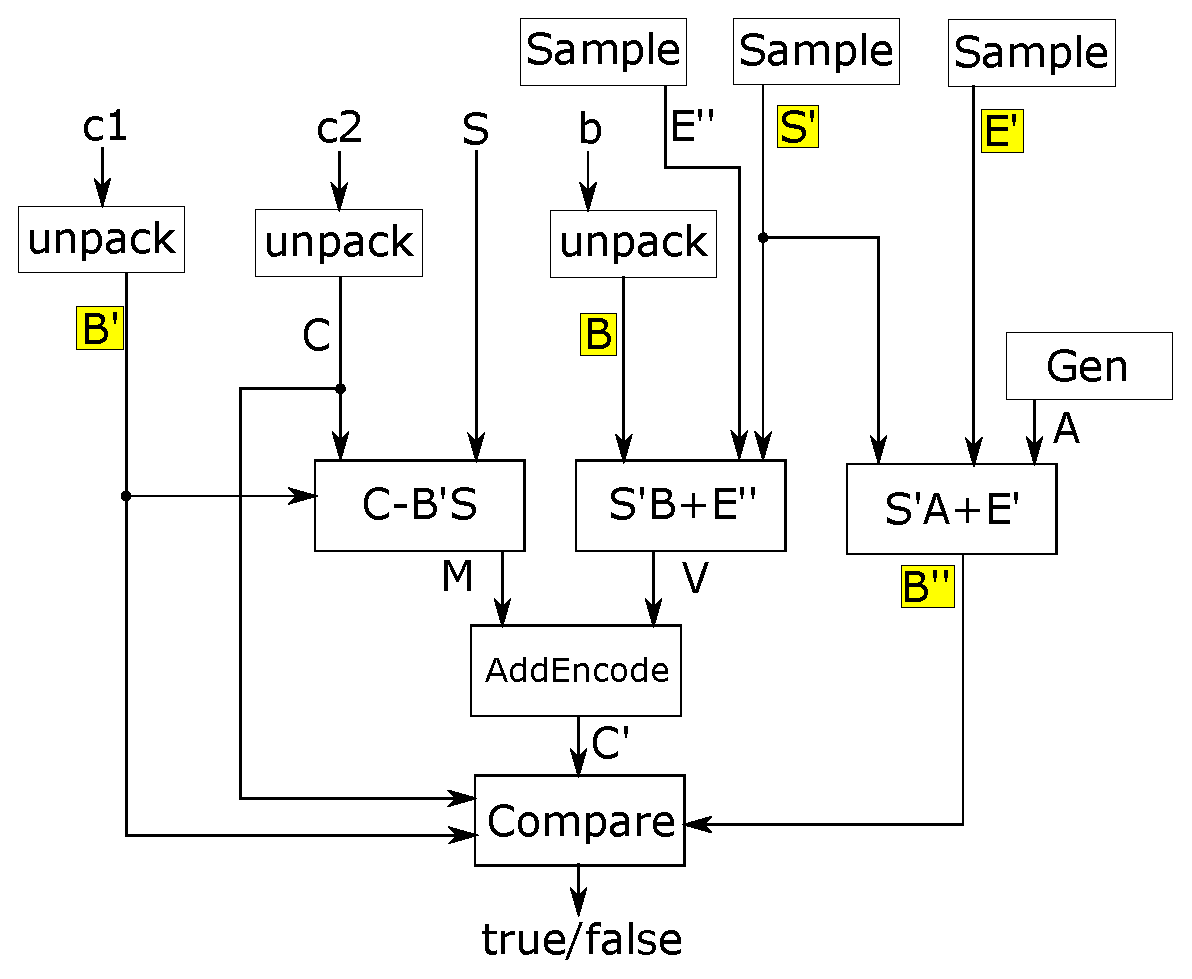
\includegraphics[scale=0.6]{figures/frodo_flowchart_decaps}

\caption{Flowchart of the decapsulation. Yellow highlighted matrices are $n \times \bar{n}$ matrices.}
\label{fig:flowchart_decaps}
\end{figure*}

\subsection{Low-level Assembly Optimization}

Our measurements indicate that besides the generation of the matrix $\mathbf{A}$, the multiplication of $\mathbf{A}$ with the secret matrix consumes most of the cycles, and therefore optimizing the multiplication is profitable. The simple operation of multiplication consumes just a small part of the cycles, the loading and storing of the matrix entries is the decisive part. Therefore minimizing the memory accesses is the key to a short run-time. Since the generation of the matrix $\mathbf{A}$ needs to be computed on-the-fly due to the memory constraints on the ARM Cortex-M4F, the multiplication cannot be done on the whole matrix $\mathbf{A}$ at once. We chose to generate $\mathbf{A}$ row-by-row when computing $\mathbf{AS}$. For the computation of $\mathbf{S'A}$ the generation of $\mathbf{A}$ depends on the choice of the permutation function. Writing the multiplication in assembly language gives us more control over the implementation and allows us to incorporate enhancements the compiler cannot engineer. Since the amount of memory accesses is substantial for the speed, our goal is to load the necessary matrix entries from RAM as rarely as possible and use all the available registers.

When $\mathbf{A}$ is generated on-the-fly, a straightforward implementation of the multiplication of $\mathbf{AS}$ has two loops. The first loop iterates over the columns of $\mathbf{S}$ with $\bar{n}$ iterations. The second loop iterates over the rows of $\mathbf{S}$, respectively the entries of the generated row of $\mathbf{A}$ with $n$ iterations.  But as $\bar{n} = 8$ in both parameter sets, it is possible to implement the matrix multiplication by using only one loop. During the multiplication of one row of $\mathbf{A}$ with $\mathbf{S}$, only eight entries of $\mathbf{AS}$ are computed. Since these entries are the sum of the products of $n$ multiplications, they are often updated during the computation. Storing the eight entries of $\mathbf{AS}$ in registers during the whole computation enables us to save many memory accesses: instead of iterating over the eight columns of $\mathbf{S}$, it is possible to process one entry of $\mathbf{A}$ with a complete row from $\mathbf{S}$ during one iteration. Figure \ref{fig:mul} presents this concept graphically.

  \begin{figure}[tbhp]
  	\centering
  	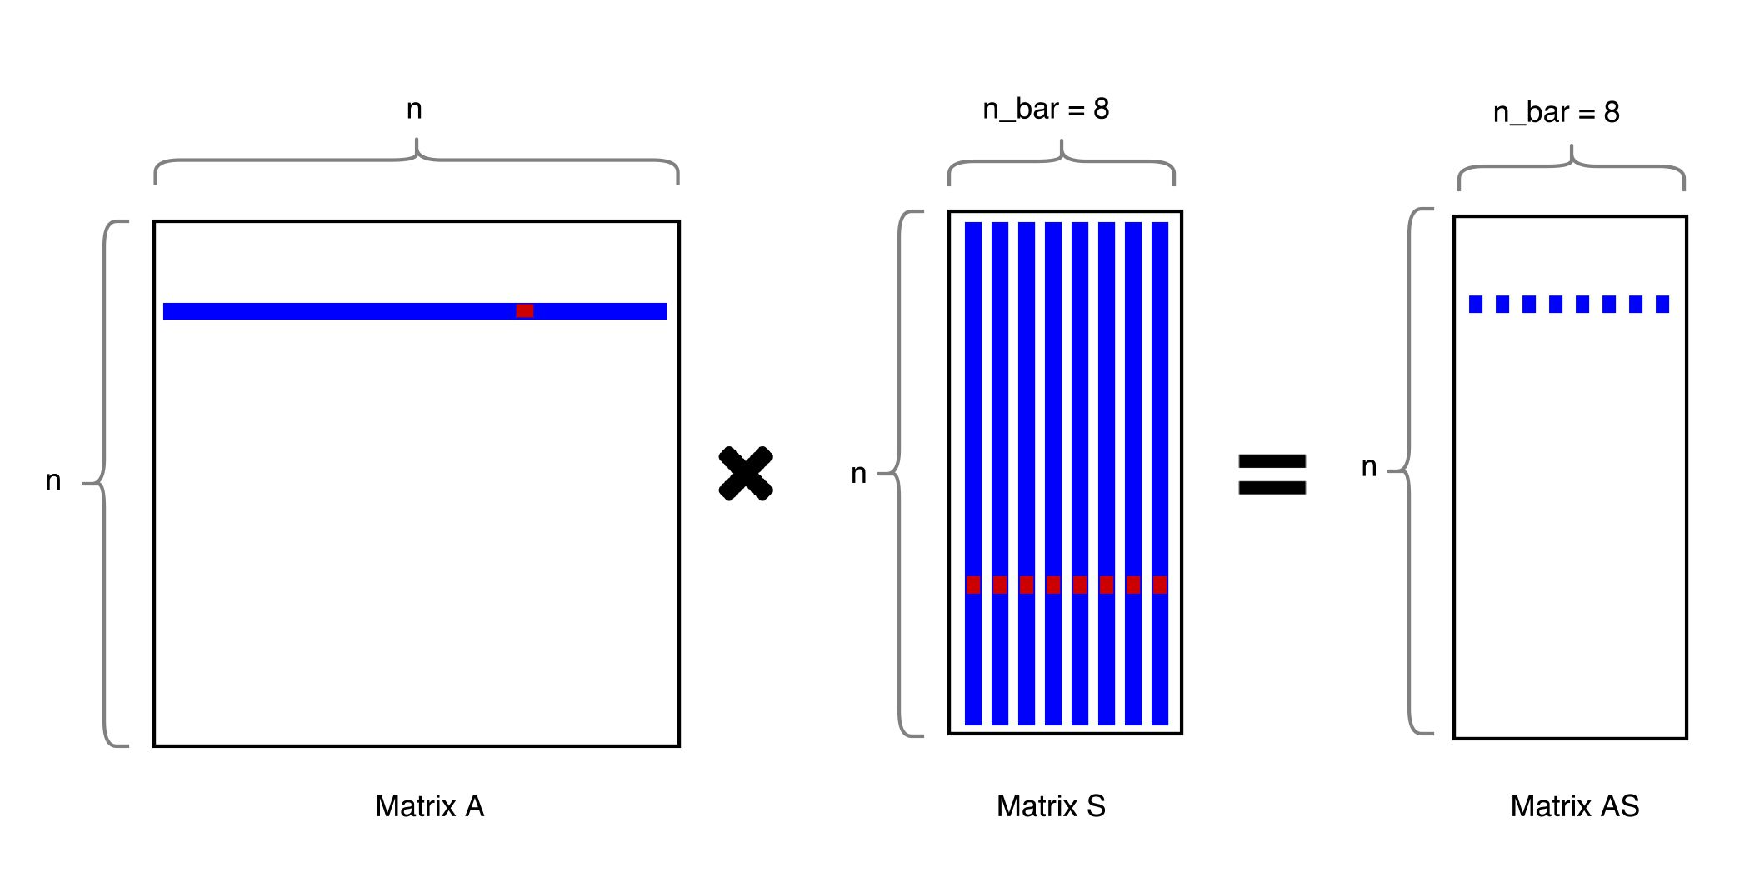
\includegraphics[width=1\textwidth,]{figures/mul.pdf}
  	\caption{Concept of the multiplication of one row of $\mathbf{A}$ with $\mathbf{S}$ effectively. Blue entries are affected by one function call, red entries are loaded during one iteration.}
  	\label{fig:mul}
  \end{figure}

The multiplication of $\mathbf{A}$ and matrix $\mathbf{S'}$ is slightly different, and variates with the use of either AES or cSHAKE. With cSHAKE, the matrix $\mathbf{A}$ is intended to be generated only in entire rows, which is convenient for the computation of $\mathbf{AS}$, but inefficient for the computation of $\mathbf{S'A}$, because one row of $\mathbf{A}$ affects all elements of $\mathbf{S'A}$. 
With AES, $\mathbf{A}$ is generated in blocks of 128 bits, therefore it is not only possible to generate $\mathbf{A}$ row-by-row but also by producing eight columns at a time. In a straightforward implementation, this leads to a third  loop iterating over the eight columns. The fact that the number of processed columns of $\mathbf{A}$ is eight, just as the parameter $\bar{n}$, enables us to use the same concept that we used for the multiplication of $\mathbf{S'A}$. We illustrate this concept in Figure \ref{fig:mulcol}. To avoid nested loops, we unroll the loop that gets added due to the eight columns. We end up with eight loops that are run through \emph{after} each other.
	
 \begin{figure}[tbhp]
   	\centering
   	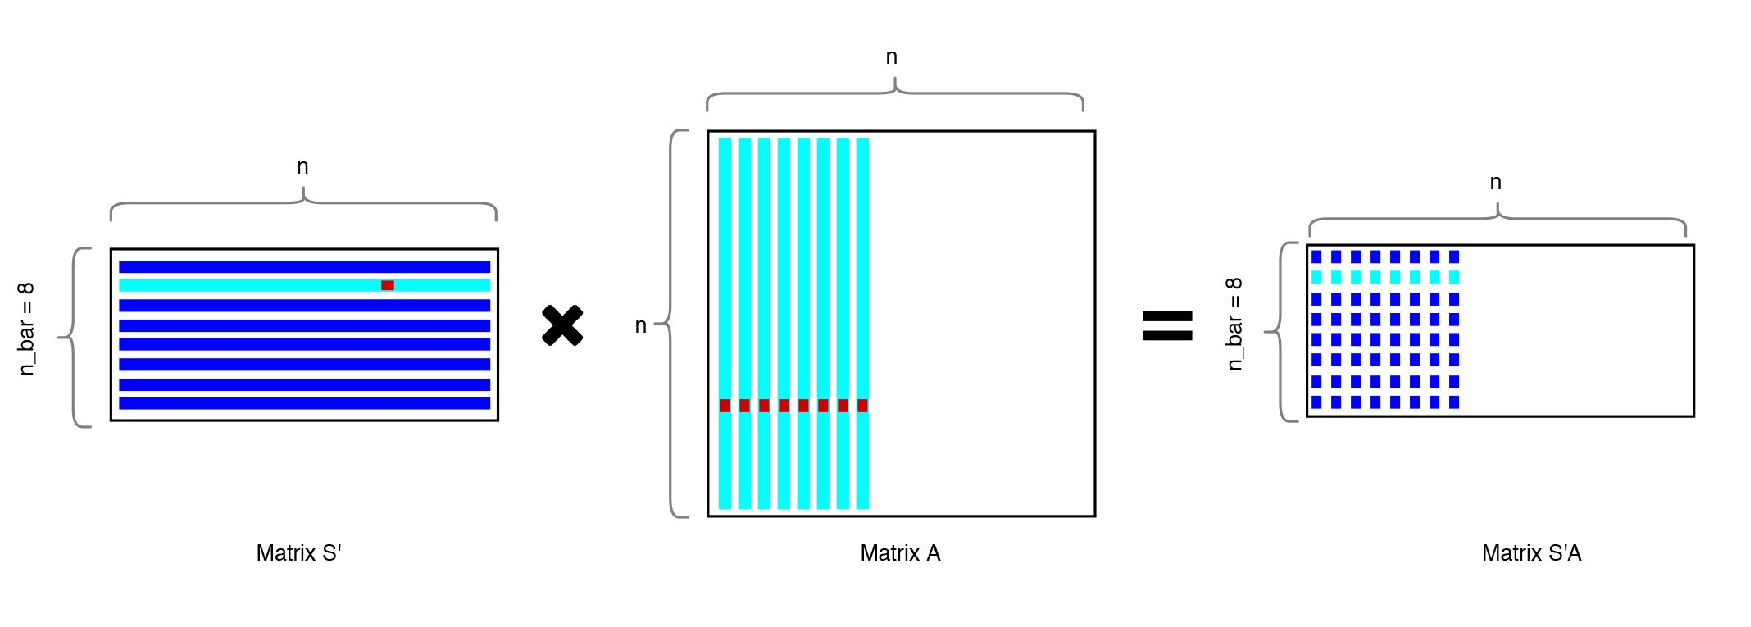
\includegraphics[width=1\textwidth,]{figures/colmul.pdf}
   	\caption{Concept of the multiplication of 8 columns of $\mathbf{A}$ with $\mathbf{S'}$ effectively. Blue and light blue entries are affected by one function call, light blue entries are loaded by one entire loop, red entries are loaded during one iteration.}
   	\label{fig:mulcol}
 \end{figure}

The ARM Cortex-M4F offers 13 general purpose registers $R0-R12$ which we use all in our assembly matrix multiplication to maximize memory efficiency. Furthermore we use the designated link register $R14$ whose content we preserve on the stack. In $R0$ a pointer to matrix $\mathbf{A}$ is passed, in $R1$ a pointer to matrix $\mathbf{S}$, and in $R2$ a pointer to matrix $\mathbf{B}$. After loading the eight relevant entries of $\mathbf{B}$ into the registers $R4-R11$, we use $R2$ to store elements of $\mathbf{A}$. In $R3$ we pass the parameter $n$, which defines the number of iterations through the loop. In $R12$ and $R14$ entries of $\mathbf{S}$ are stored.

In both parameter sets, entries of matrices are stored in 16-bit data types, but the ARM Cortex-M4F is a 32-bit architecture. This enables us to reduce memory access, by loading two entries of matrix $\mathbf{A}$ simultaneously, as in Line 1 of Listing \ref{lst:loop1}. In the next line we use an instruction to load multiple aligned words, to get four entries of $\mathbf{S}$ by only one instruction. The single-cycle multiply-with-accumulate capabilities are very valuable for the actual matrix multiplication, used for example in Line 3 of Listing \ref{lst:loop1}.

\begin{lstlisting}[caption={Multiplication in Assembly}\label{lst:loop1}]
ldr r2, [r0], #4     //r2=a_ij+1, a_ij
ldmia r1!, {r12,r14} //r12=s_ij+1, s_ij, r14=s_ij+3,s_ij+2
mla r4, r2, r12, r4  //r4=r2*r12+r4
lsr r12, r12, #16    //r12=s_ij+1
mla r5, r2, r12, r5
mla r6, r2, r14, r6
lsr r14, r14, #16
mla r7, r2, r14, r7
\end{lstlisting}

\subsection{Protection Against Timing Side Channels}
Our implementations using cSHAKE have a constant timing and are therefore protected against timing attacks. The AES implementation from \cite{DBLP:conf/sacrypt/SchwabeS16} is very efficient but due to the caches on our development board not timing-constant. Therefore we disabled the data and instruction cache by clearing bit 9 and bit 10 of the \texttt{FLASH\_ACR} register. We noticed only a negligible drop in performance ($< 1$\%) after disabling the caches.
